\newpage
\section{Design}
\label{design}

Für das Design der Webseite werden überwiegend grau/weiße Boxen verwendet. Diese sehen wie folgt aus:

\begin{figure}[H]
    \begin{center}
      \frame{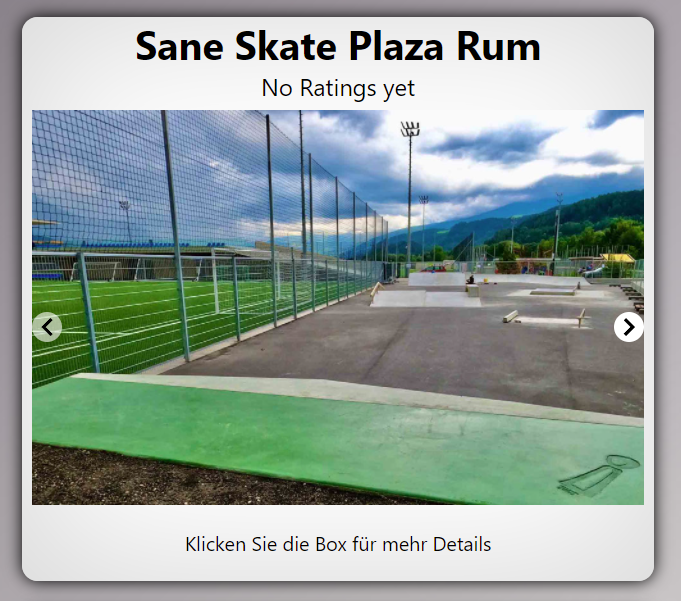
\includegraphics[width=0.8\textwidth]{Website/Box.png}}
      \caption{CSS Boxen}
    \end{center}
\end{figure}

Diese Boxen haben einen einheitlichen CSS Code damit sie auf jeder View gleich aussehen.

\begin{code}[htp]
\begin{lstlisting}
    display: block;
    margin: 5% auto;
    border-radius: 2vh;
    box-shadow: inset 0 0 10em lightgray, 0 0 1em black;
    background-color: white;
    margin-top: auto;
    margin-bottom: auto;
    min-height: 70vh;
\end{lstlisting}
\caption{CSS - Boxen}
\end{code}

Die Box besteht also aus einen einfachen Border mit einem Schatten. Damit die Ecke rund sind,
ist der Radius des Borders 2vh groß. Vh ist eine Einheit, welche sich auf die Höhe des Bildschirmes 
anpasst. 2vh bedeuten 2\% der Bildschirmhöhe. 